



\usepackage{algorithm}%,algpseudocode}
\usepackage{mdframed}

%\def\input@path{{/figures/}}
%\def\input@path{{/path/to/folder/}{/path/to/other/folder/}}

\newcounter{algsubstate}
\renewcommand{\thealgsubstate}{\alph{algsubstate}}
\newenvironment{algsubstates}
  {\setcounter{algsubstate}{0}%
   \renewcommand{\State}{%
     \stepcounter{algsubstate}%
     \Statex {\footnotesize\thealgsubstate:}\space}}
  {}


\numberwithin{equation}{section}
\usepackage[labelfont=bf, font=it]{caption}
\captionsetup{width=0.6\textwidth}
\usepackage{here}
%\newcommand{\showothermaterial}{this}
%\usepackage{kpfonts}
%\usepackage{hyperref}
\usepackage{framed}
%\usepackage{listings}
\usepackage{bbm}
%\usepackage{color}
%%\usepackage{autoref}
%\usepackage{tikz}\
\usepackage{graphicx}
\graphicspath{{figures/}{../../figures/figures-static/}}
\usepackage{wasysym}
\usepackage{tgbonum}
\usepackage{multicol}
\usepackage{pdfpages}
\usepackage{pgfplots}
\usepackage{algorithm}
\usepackage[noend]{algpseudocode}
\renewcommand{\algorithmicrequire}{\textbf{Input: }}
 \renewcommand{\algorithmicensure}{\textbf{Output: }}
 
%\usetikzlibrary{shapes.arrows}
%\usetikzlibrary{backgrounds}
%\usetikzlibrary{positioning}
%\usetikzlibrary{arrows}
%\definecolor{gray}{gray}{0.3}
%\definecolor{darkgreen}{rgb}{0,0.55,0}
%\definecolor{purple}{rgb}{0.5,0,1}
%
%\oddsidemargin=0in
%\evensidemargin=0in
%\textwidth=6.5in
%\topmargin=-1in
%\textheight=25cm
%\parindent=0in
\usepackage{calc}
\newsavebox\CBox
\newcommand\hcancel[2][0.5pt]{%
  \ifmmode\sbox\CBox{$#2$}\else\sbox\CBox{#2}\fi%
  \makebox[0pt][l]{\usebox\CBox}%  
  \rule[0.5\ht\CBox-#1/2]{\wd\CBox}{#1}}

\usepackage{xcolor}
\colorlet{notgreen}{blue!50!yellow}
\newcommand{\tblue}[1]{{\color{blue} #1}}
\newcommand{\tred}[1]{{\color{red} #1}}
\newcommand{\tgreen}[1]{{\color{notgreen} #1}}

\newcommand{\code}[1]{\texttt{ #1}}
\newcommand{\complexity}[1]{{\color{red} \textit{#1}}}
\newcommand{\nphard}{\complexity{NP-Hard}}
\newcommand{\npcomplete}{\complexity{NP-Complete}}
\newcommand{\polynomial}{{\color{ansi-green} \textit{Polynomial time (P)}}}
\newcommand{\true}{\tgreen{\texttt{ true }}}
\newcommand{\false}{\tred{\texttt{ false }}}

\usepackage{scalerel}
\newcommand{\julia}{\raisebox{-.2\height}{
\includegraphics[scale = 0.07]{julia-logo}}  }
\newcommand{\jupyter}{\raisebox{-.2\height}{
\includegraphics[scale = 0.09]{jupyter-logo}}  }
\newcommand{\jump}{\raisebox{-.2\height}{
\includegraphics[scale = 0.08]{jump-logo}}  }
\newcommand{\gurobi}{\raisebox{-.2\height}{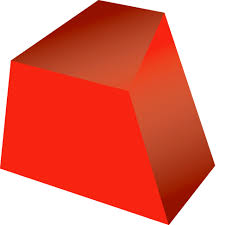
\includegraphics[scale = 0.06]{gurobi-logo}}Gurobi  }
\newcommand{\coin}{\raisebox{-.2\height}{
\includegraphics[scale = 0.2]{coin-or-logo}}  }
\newcommand{\ipopt}{\raisebox{-.2\height}{\texttt{Ipopt}}}


\usepackage{subcaption}

\def \PP{ {\mathcal{P}}}
\def \NN{ {\mathcal{N}}}
\def \II{ {\mathcal{I}}}
\def \ZZ{ {\mathcal{Z}}}
\def \SS{ {\mathcal{S}}}
\def \FF{ {\mathcal{F}}}
\def \CC{ {\mathcal{C}}}
\def \nn{ {\mathbb{N}}}
\def \R{ {\mathbb{R}}}
\def \Z{ {\mathbb{Z}}}
\def \Q{ {\mathbb{Q}}}
\def \cc{ {\mathbb{C}}}

\DeclareMathOperator{\dom}{dom}
\DeclareMathOperator{\cl}{cl}
\DeclareMathOperator{\intr}{intr}

\def \rank{\textup{rank}}
\def \size{\textup{size}}
\def \dist{\textup{dist}}
\def \sign{\textup{sign}}
\def \deg{\textup{deg}}
\def \conv{\textup{conv}}
\def \cone{ {\textup{cone}}}
\def \supp{\textup{supp}}
\def \int{ {\textup{int}}}
\def \rc{\textup{rec.cone}}
\def \ri{\textup{rel.int}}
\def \rb{ {\textup{rel.bd}}}
\def \bd{ {\textup{bd}}}
\def \ls{\textup{lin.space}}
\def \tq{{\,:\,}}
\def \aff{{\textup{aff}}}
\def \one{\mathbbm{1}}
\def \st{ \text{ s.t. }}

\def \BQP{\mathrm{BQP}}
\def \xLP{x^{\mathrm{LP}}}
\DeclareMathOperator    \argmin         {arg\,min}
\DeclareMathOperator    \argmax         {arg\,max}



\newcounter{example}
\newcounter{general}

  % Test Environment
  \newcounter{exo}
\makeatletter
\newenvironment{exo}[1]%
{\refstepcounter{exo}%
\protected@edef\@currentlabelname{Exercise \theexo: #1}% addition here
\vspace{0.5cm}\noindent
{\large\bfseries{Exercise \theexo~: #1} \par}
{\par\vspace{0.5cm}}}
\makeatother

\newcounter{codeCell}
\makeatletter
\newenvironment{codeCell}%
{\refstepcounter{codeCell}%
\protected@edef\@currentlabelname{Code}% addition here
{}
%{\large\bfseries{Exercise \theexo~: #1} \par}
{}}
\makeatother

% General environment
\newenvironment{general}[2]
  {\par\medskip
   %\refstepcounter{exo}%
  \protected@edef\@currentlabelname{#1}
   \begin{framed}
   \begingroup\color{black}%
   \textbf{#1: }\ignorespaces
   \par #2
   \par}
 {\endgroup\end{framed}
  \medskip}
  

 % Example Environment
  \newenvironment{example}
  {\par\medskip
  \refstepcounter{exo}%
  \protected@edef\@currentlabelname{Example \theexo}
   \begin{framed}
   \begingroup\color{blue}%
   \textbf{Example \theexo: }\ignorespaces}
 {\endgroup\end{framed}
  \medskip}
  
  
  % Example with code Environment
   \newenvironment{examplewithcode}[2]
  {\par\medskip
   \refstepcounter{exo}%
  \protected@edef\@currentlabelname{Example \theexo}
   \begin{framed}
   \begingroup\color{blue}%
   \textbf{Example: #1}
   \hfill
    [Code: \autoref{#2}]\ignorespaces
    \par}
 { \endgroup
 \end{framed}
  \medskip}
  
  
    \newcounter{todo}
    % Example with code Environment
   \newenvironment{todo}
  {\par\medskip
   \refstepcounter{todo}%
  \protected@edef\@currentlabelname{To Do: \thetodo}
   \begin{mdframed}[backgroundcolor=yellow!20,nobreak=true] 
   \begingroup\color{red}
   \textbf{To Do \#\thetodo:}
   }
 { \endgroup
 \end{mdframed}
  \medskip}
  
  
  
  
  %\usepackage{subfiles}
\usepackage{amsthm,amsfonts,amsmath,amstext,amssymb,amsopn}
\usepackage{tkz-graph}
\usetikzlibrary{plotmarks,trees,arrows}
\usetikzlibrary{graphs,graphs.standard}
\usepackage[cc]{titlepic}
\usepackage{longtable}
\usepackage{pgfplots} 
\pgfplotsset{compat=newest}
\pgfplotsset{plot coordinates/math parser=false}
\pgfplotsset{
    every non boxed x axis/.style={
        xtick align=center,
        enlarge x limits=true,
        x axis line style={line width=0.8pt, -latex}
},
    every boxed x axis/.style={}, enlargelimits=false
}
\pgfplotsset{
    every non boxed y axis/.style={
        ytick align=center,
        enlarge y limits=true,
        y axis line style={line width=0.8pt, -latex}
},
    every boxed y axis/.style={}, enlargelimits=false
}
\usetikzlibrary{
   arrows.meta,
  intersections,
}
\tikzset{>=latex}

%\usepackage{amsmath}
\usepackage{pgfplots}
\usepgfplotslibrary{fillbetween}
%\usetikzlibrary{arrows.meta}


\usepackage{pythontex}
\newtheorem{theorem}{Theorem}
\newtheorem{lemma}[theorem]{Lemma}
\newtheorem{exercise}[theorem]{Exercise}
\newtheorem{proposition}[theorem]{Proposition}
\newtheorem{definition}[theorem]{Definition}
\newtheorem{remark}[theorem]{Remark}
\usepackage[subpreambles=false]{standalone}
\usepackage{import}

\usepackage{subfiles}

\usepackage{animate}
  